\documentclass[12pt,letterpaper,oneside]{book}
\usepackage{afitStyleFiles/afitThesis}
\usepackage{xcolor}
\usepackage{soul}
\usepackage{sf298}
\usepackage{tabularx}
\usepackage{multirow}
\usepackage{pdfpages}
\usepackage[all]{nowidow}
\usepackage{gensymb}
\usepackage{IEEEtrantools}
\usepackage{multirow}
\usepackage{bm}
\usepackage{url}
\def\UrlBreaks{\do\/\do-}
\usepackage[breaklinks]{hyperref}


\afitthesis %%default
% \afitreport
% \dissertation
% \prospectus

\def\author{Sean R. Kelly}

\rank{Capt, USAF} 

\docdesignator{AFIT-ENV-MS-21-M-???}
\department{Department of Systems Engineering and Management}
\graduationdate{March 2021}


\flytitle{\MakeUppercase{Developing a CubeSat Reference Architecture}}
\title{\MakeUppercase{Developing a CubeSat Reference Architecture}}

\previousdegrees{BS}
\acdegree{Master of Science in Systems Engineering}
 
\committee{{David R. Jacques, Ph.D.\\Chair},
            {Thomas C. Ford, Ph.D.\\Chair}
            {Richard G. Cobb, Ph.D.\\Member},
            {Bradley J. Ayres, Ph.D.\\Member},
}

\address{2950 Hobson Way\\ Air Force Institute of Technology \\
Wright-Patterson AFB, OH 45433}

\distribution{DISTRIBUTION STATEMENT A\\[-10pt]
\MakeUppercase{Approved for Public Release; distribution unlimited.}
} 


\disclaimer{The views expressed in this document are those of the
author and do not reflect the official policy or position of the
United States Air Force, the United States Department of Defense or
the United States Government.  This material is declared a work of the
U.S. Government and is not subject to copyright protection in the
United States.}
%% myFigures.tex
% A common file to store all figure definitions
%
% In preparing your thesis, one of the first things you should do is
% organize your figures.  Then, one of the last things you'll do is
% reorder your figures so they display where you want them to in the
% text.  Organizing figure definitions in a common files helps:
%
%   1. Write new figures using earlier examples.
%
%   2.  Isolate code and minimize the risk of introducing bugs in the
%   final editing process.  Trust me, moving around just one line of
%   code is easier.
%
%   3.  Reuse figures in other papers.  <=== the best reason!
%
% Note command names can not include numbers and special characters.
%
% To make the file more searchable, use naming conventions that map
% the graphics filename labSetup.jpg to the command name \figlabSetup to the
% figure label fig:labSetup.
% 

\newcommand{\figMyFirstLaTeX}{\begin{figure}[tbp]
 \begin{center}
    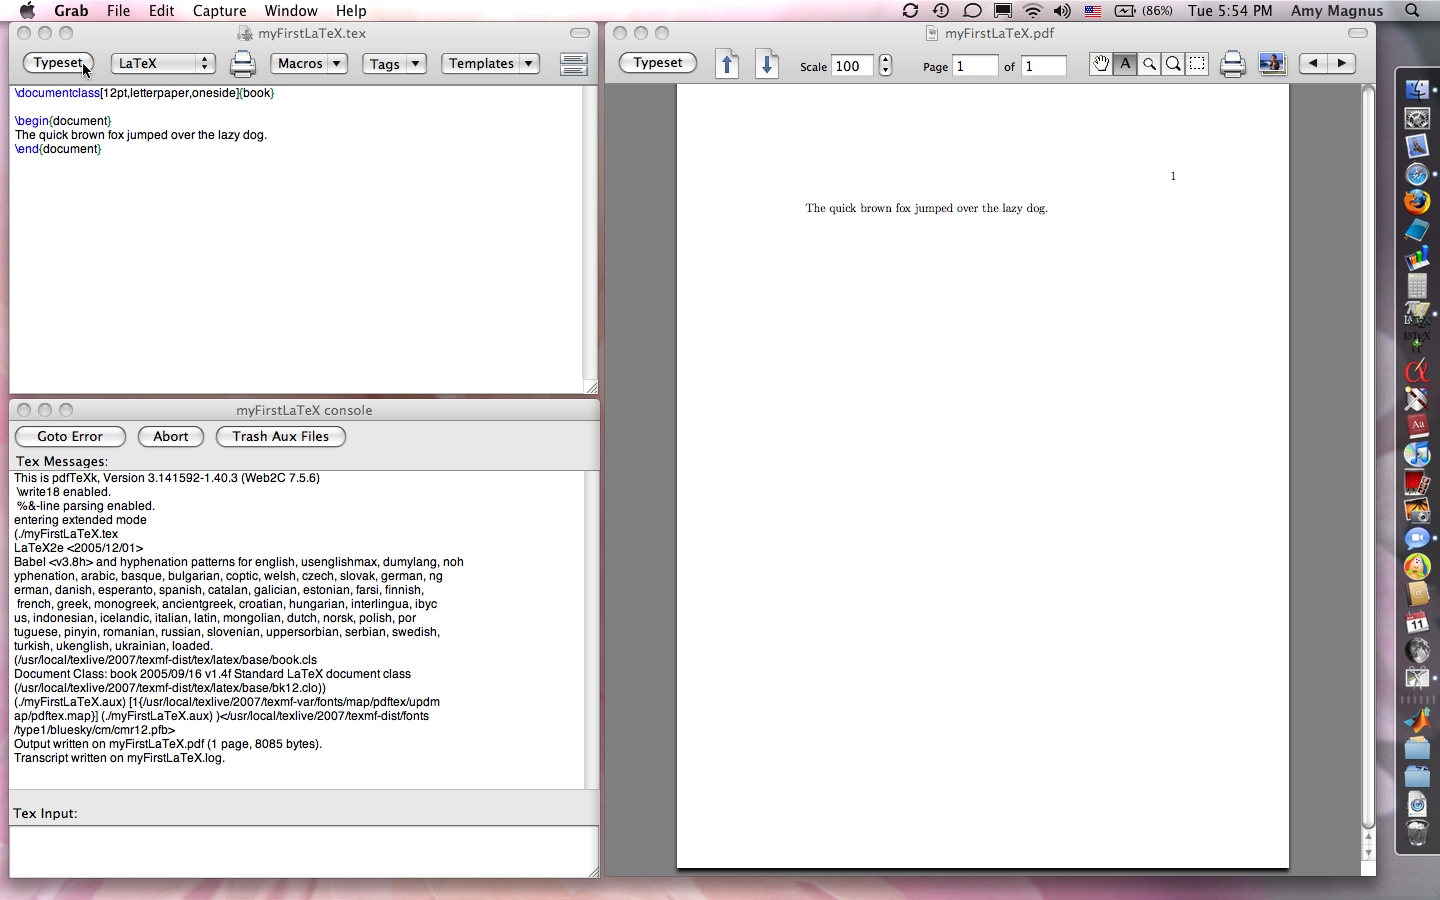
\includegraphics[width=6in]{Figures/myFirstLaTeXCursor}
     \caption[\LaTeX\ a very simple document]{Compile a very simple document.}
     \label{fig:MyFirstLaTeX}
 \end{center}
 \vspace{-0.2 in}
\end{figure}
}




%\input{Thesis/Preamble/myTables}
\def\Plus{\texttt{+ }}
\def\Minus{\texttt{- }}

\newenvironment{conditions*}
  {\par\vspace{\abovedisplayskip}\noindent
   \tabularx{\columnwidth}{>{$}l<{$} @{${}={}$} >{\raggedright\arraybackslash}X}}
  {\endtabularx\par\vspace{\belowdisplayskip}}
  
\newenvironment{conditions}
  {\par\vspace{\abovedisplayskip}\noindent\begin{tabular}{>{$}l<{$} @{${}={}$} l}}
  {\end{tabular}\par\vspace{\belowdisplayskip}}


\begin{document}
%
\frontmatter\flyleaf
    \disclaimerpage
    \titlepageAFIT
    \committeepage
    \begin{abstract}

The CubeSat class of nanosatellites has lowered the barrier of entry to space and has rapidly gained popularity in recent years. The lower development cost, small form factor, and reuse of commercial off-the-shelf components makes the CubeSat form factor an ideal platform for University teams, where budget and development time are extremely limited. To successfully design a CubeSat system in a rapid cycle conducive to academic timelines, a Reference Architecture geared towards University CubeSat development would be helpful. A Reference Architecture would speed up the development process by providing a template, capturing previous work and lessons learned from subject matter experts, providing a framework to focus on the CubeSat’s design rather than the fine details of modeling software. A Reference Architecture can also add functionality that student teams could use and improve over time, such as pre-built analysis functions and a library of components to choose from. This thesis presents a CubeSat Reference Architecture designed to meet these needs and explores its unique features, diagrams, and custom libraries. The CubeSat Reference Architecture was validated by relevant course instructors and is being used by a cohort of students in the Spacecraft Design Sequence at AFIT.


\end{abstract}
    \begin{acknowledgements}


I would like to express my sincerest appreciation to my committee members for their guidance through this process. Dr. Jacques and Dr. Cobb, I thank you for your .............(finish this at the end)

\vspace*{20mm}

\hspace*{7cm} Sean Kelly
\end{acknowledgements}

    \tableofcontents
    \listoffigures
    \listoftables
    \listofabbreviations

\mainmatter
	\chapter{Introduction}
    \label{Intro}
    	\section{General Issue}
   		\label{geniss}
    	Designing a spacecraft is a daunting and complex endeavor. Due to the nature of space launch, most spacecraft only get one chance at success, and spacecraft can take many years and millions of dollars to develop. As such, modeling, simulation, and testing are vital for a space vehicle program's success, and finding new ways to mature technologies and flight test them can improve this process. The CubeSat-class of nanosatellite can help by providing a cost-effective platform to mature technologies or even perform operational missions as part of a CubeSat constellation. This thesis attempts to assist design teams in rapidly developing and prototyping these CubeSat designs. 

Dr. Will Roper, assistant secretary of the Air Force for acquisition, has emphasized the need for a faster acquisition cycle and for bolder ideas. During the Air Force Association’s Air, Space and Cyber Conference in 2019, Dr. Roper said “To become a more competitive acquisition system, the Air Force needs to be aware of trends in technology. The world is changing. We have to change with it. The key is to decide which technology will be successful and being able to act on those trends with a system that is leaner, meaner and faster than our opponents.” \citep{Roper2019} In the space domain, CubeSats are that latest technological "leaner and meaner" trend, and the US Air Force and Space Force are embracing it. Additionally, CubeSats are becoming increasingly popular  in the commercial sector around the world, with the number of CubeSat launches increasing year over year.

To support research in this CubeSat domain, the \abbreviationFull[Air Force Institute of Technology]{AFIT} has a space vehicle design series of courses that guides students through the Systems Engineering process using a satellite system. Starting with a set of mission objectives, the design teams perform trade studies, generate requirements, design the CubeSat system, and perform verification and validation of those requirements with physical components over the span of three courses. This process mirrors the real-world development process, but on a much faster timeline. 

As design teams begin the development process of a CubeSat, there can be a steep learning curve. Many engineers are not familiar with \abbreviationFull[Model-Based Systems Engineering]{MBSE} tools or methodologies, and teams need to start their designs from scratch. Reference Architectures exist in other domains to capture best practices and provide a starting point for new systems, so this thesis attempts to develop and demonstrate a Reference Architecture for the CubeSat domain. By providing CubeSat designers with a template, including automatically generating tables and documentation, they can focus more on the design and less on learning how to use and organize the complicated model. Additionally, by providing a component library to use and pre-built analysis tools using those components, they can build off previous successful designs and rapidly simulate candidate solutions. Thorough documentation and guidance included in the Reference Architecture will also increase standardization amongst the team. 


    	
    	\section{Problem Statement}
   		\label{probst}
    	%Problem Statement
(if it should be a short statement)
There is a need for a Reference Architecture to allow design teams to rapidly develop, simulate, and test CubeSat designs and generate traditional documentation, all from one \abbreviationFull[Model-Based Systems Engineering]{MBSE} tool.

(if it should be a Problem Description instead)
As design teams begin the development process of a CubeSat, there is a steep learning curve for many. Many engineers are not familiar with MBSE tools or methodology, and teams need to start their designs from scratch. Reference Architectures exist in other domains to capture best practices and provide a starting point for new systems, so this thesis attempts to develop and demonstrate a Reference Architecture for the CubeSat domain. By providing CubeSat designers with a template, including automatically generating tables and documentation, they can focus more on the design and less on learning how to use and organize the complicated model. Additionally, by providing a component library to use and pre-built analysis tools using those components, they can build off previous successful designs and rapidly simulate candidate solutions. Thorough documentation and guidance included in the Reference Architecture will also increase standardization amongst the design team. 
    	
    	\section{Scope}
        \label{Scope}
        %This is the scope assumption 
This research was primarily intended to aid student design teams in a University setting, and AFIT's space vehicle design series of courses is an appropriate test-bed for this. AFIT's first space vehicle design course teaches and implements MBSE for stakeholder analysis and requirements generation; however, the following courses do not continue the use of the model for the actual design and implementation of the CubeSat. The goal of this research is to create a useful Reference Architecture to aid students in designing the physical satellite and tracing system requirements down to the component level. This Reference Architecture should be useable even by users not so familiar with MBSE, and it should assist with the system-level review process including Critical Design Reviews, Test Readiness Reviews, etc. Even though AFIT students will be the first users of this Reference Architecture, it is generic enough to be used for any team wishing to develop a CubeSat program from the ground up. It has all the functionality needed to develop requirements, design the physical system, and perform basic simulations. It also features helpful resources like a component library to assist with the physical design and document generators to create tailored stakeholder documents from model elements. This CubeSat Reference Architecture is intended to model the CubeSat system, with only minimal modeling for external systems such as the ground stations. Ground station characteristics are necessary for some communications analysis, so some basic ground station modeling is included, but the ground station is not the system of interest. Other external systems, such as the launch vehicle, are also included just to document interactions as needed, but are not extensively modeled.

A Reference Architecture offers a baseline template for students to build from, using lessons learned from past projects and creating the framework to streamline the design process. A large effort of this research was focused on creating a generic model with default component specifications throughout. This was intended to spark ideas in the brainstorming process for students and aid in system analysis. Another component of this research was creating basic analysis capabilities within the model, allowing students to tweak component specifications to see how those changes affect overall capabilities and requirements. Additionally, the model traces the analysis to template requirements that future teams will tailor for their unique projects. This allows for rapid simulations of key performance parameters or measures of effectiveness for the system. Additional work is being done using this Reference Architecture for more in-depth state analysis and integration with \abbreviationFull[Systems Tool-Kit]{STK} and MATLAB, so it's critical to form a robust baseline to build off of.

In order to test the validity of the tool, examples of this Reference Architecture will first be demonstrated to the relevant course instructors to show how it could be used by students. Feedback will be incorporated into the model before being used by future classes. Additionally, a comprehensive how-to guide and modeling style guide will be provided to students to walk through the process using a generic design. 

        
    	\section{Research Objectives and Questions}
    	\label{ObjandQs}
        In an effort to improve this rapid-prototyping environment, this thesis demonstrates the usage of a new Reference Architecture to guide CubeSat design teams through the whole design process, hopefully speeding up the process and improving the quality of designs in the end. The first usage of this Reference Architecture will be the AFIT space vehicle design series, but the Reference Architecture should be useful to any CubeSat design team as a starting template. \\

\noindent \textbf{The research objectives are:}

\begin{enumerate}
\item{Create a practical and useful Reference Architecture for rapidly-prototyping CubeSat designs.}
\item{Create easy-to-use document generators that use model elements to generate traditional system level review documentation.}
\item{Present this Reference Architecture to AFIT instructors for feedback.}
\item{Lay the groundwork for future analysis work with STK and MATLAB integration for more comprehensive mission analysis using model elements.}
\end{enumerate}

\noindent \textbf{The research questions are:}

\begin{enumerate}
\item{What are the tools necessary to perform mission modeling using model-based systems engineering?}
\item{What viewpoints are most useful to common stakeholders?}
\item{How can useable documentation be generated from only model elements, keeping the source of truth within the model?}
\item{What needs to be done in the model to allow for external tools (STK, MATLAB, etc.) to interact with the MBSE tool?}
\item{Can cloud-based collaboration improve the MBSE design process for interdisciplinary teams?}

\end{enumerate}
        
        \section{Assumptions and Limitations}
        \label{Assums_Limits}
        % Assumptions and Limitations

% Think of implicit assumptions and make explicit by stating them here
    
There are of course some limitations to this research. The first is limited standardization amongst the CubeSat community. This thesis is based on how AFIT teaches MBSE and how AFIT names subsystems, requirements, and documents. Other design teams may have vastly different practices and conventions, limiting how useful the Reference Architecture may be right away. Second, this Reference Architecture uses Cameo Systems Modeler, a tool that might not be available or desired by users. Third, the Reference Architecture is sensitive to major organizational changes. If a user wishes to make drastic changes away from the provided structure, some analysis or document tools may need to be updated or they will not be useful. Finally, the analysis portion of this Reference Architecture is only useful for initial verification and validation of requirements, but does not replace more in-depth and robust analysis. This tool can help rapidly prototype and determine feasibility, but would not suffice for final approval to launch. 
        
        \section{Preview}
        \label{preview}
        %The preview section of the introduction
The thesis follows a five-chapter format. Chapter \ref{Intro} presented the general issue, listed the research goals, provided the scope and general approach of this research, and listed assumptions and limitations. Chapter \ref{LitReview} provides a background on the current Reference Architectures in the CubeSat domain and how other Reference Architectures are being used in other fields. Chapter \ref{Methodology} describes the methodology used to address the problem statement and complete the research objectives. Chapter \ref{analysis} details the resulting Reference Architecture and accompanying analytical tools. Chapter \ref{conclusion} summarizes the contributions and limitations, and describes areas of future research to further refine and evolve the Reference Architecture’s usefulness. 

Ultimately, the final objective of the thesis effort is to provide CubeSat designers and students with a useful baseline on which to design a system that meets mission requirements. Furthermore, those requirements should be validated at the logical and hardware levels using tools such as STK and MATLAB.

	\chapter{Literature Review}
    \label{LitReview}
 
        \section{Overview}
        \label{LitOver}
   		The purpose of this chapter is to highlight the current state of Reference Architectures, including some recent work in the CubeSat domain. To understand the context, this chapter will start by describing the CubeSat domain and the need for a CubeSat Reference Architecture. This chapter will also define key terms and explore gaps in the existing CubeSat models. Reference Architectures in the CubeSat domain are still a relatively new endeavor, but Reference Architectures in similar domains will be researched to learn lessons from those models as well. 

        
        \section{CubeSats}
        \label{CubeSats}
   		As launch service providers continue to offer more ride-sharing opportunities, access to space has never been more available or affordable for small satellites. The nanosatellite size (1-10 kg) (cite) has exploded in popularity over the last two decades, and among that size class, the CubeSat construct has become the de facto standard. A CubeSat is a sizing standard defined in 1999 by California Polytechnic State University and Stanford University's \abbreviationFull[Space and Systems Development Laboratory]{SSDL}, with a basic "1U" unit being 10 cm x 10 cm x 10 cm and a mass less than 1.33 kg \citep{DesignSpec}. An example 1U CubeSat is shown in Figure \ref{fig:1U CubeSat Example}. Furthermore, CubeSats are defined by how many 1U cubes they contain. For example, a 3U CubeSat would be three 1U cubes together, and a 6U CubeSat is six 1U cubes combined, as shown in Figure \ref{fig:6U CubeSat Example}. This standardized sizing framework allows for rapid prototyping with common chassis and common dispenser mechanisms, and this drives down the cost of research and development for these CubeSats. CubeSats routinely use \abbreviationFull[Commercial Off The Shelf]{COTS} components to further drive down development costs. California Polytechnic Institute also publishes CubeSat Design Specifications for 1U-3U CubeSats and for 6U CubeSats to assist design teams \citep{DesignSpec}.

\begin{figure}[!h]
    \centering
    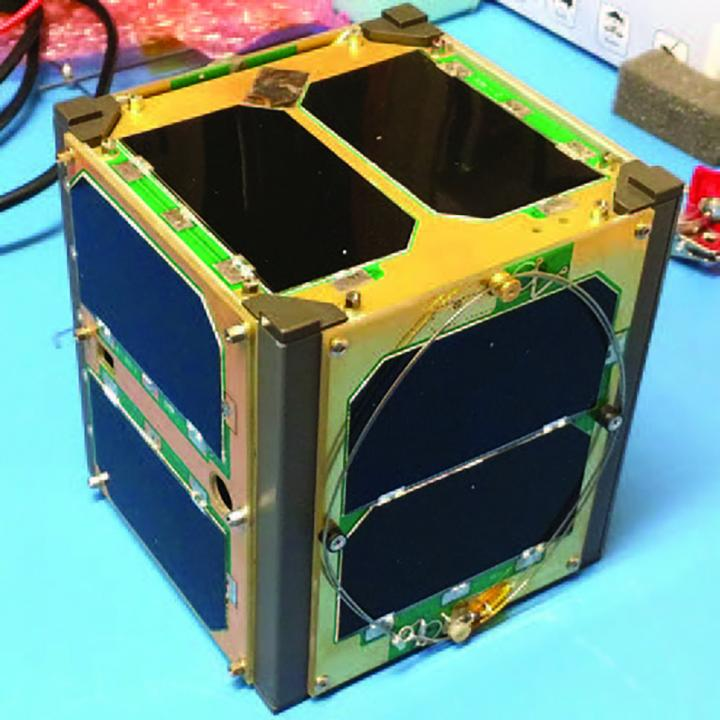
\includegraphics[width=3in]{Thesis/Literature_Review/Lit Review Figures/vanderbiltcubesat.jpg}
    \caption{1U CubeSat Example}
    \label{fig:1U CubeSat Example}
\end{figure}

\begin{figure}[!h]
    \centering
    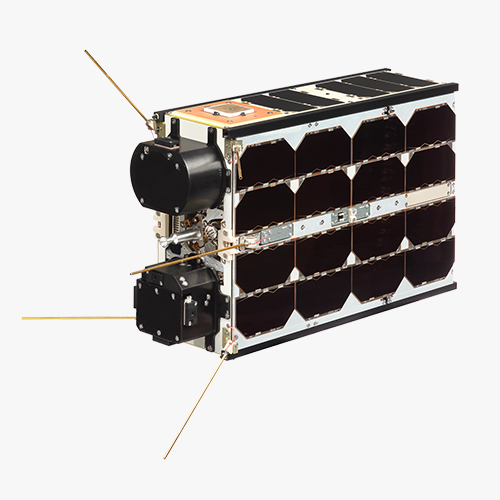
\includegraphics[width=3in]{Thesis/Literature_Review/Lit Review Figures/6Ucubesatbus.jpg}
    \caption{6U CubeSat Example}
    \label{fig:6U CubeSat Example}
\end{figure}

A primary benefit of the CubeSat standard is the lower cost of both the satellite hardware and of the launch costs. The cost of failure for a CubeSat is orders of magnitude less than for a large, exquisite satellite, so CubeSats offer a proving ground for maturing technologies. A traditional satellite requires a dedicated launch vehicle, a distinct payload adapter, and millions to billions of dollars in research and development. By contrast, a CubeSat might only cost \$100,000 to \$500,000 in research and development costs, and the launch cost can be less than \$1 Million (cite). Even more valuable than the reduced cost is the ability to flight test articles in the space environment to iterate and mature technologies. Many materials, sensors, and other components have been matured through CubeSats. For example, the Air Force Academy's FalconSat-7 was designed to get flight heritage on a polyimide photon sieve and determine its imaging performance before being used in future operational satellites \citep{FalconSat7}. Their previous mission, FalconSAT-6, was designed to improve \abbreviationFull[Hall Effect Thruster]{HET} technologies and low power communication options \citep{FalconSat6}. 

Furthermore, as resiliency in space becomes more important, CubeSats offer a solution that is attracting research for military application. As CubeSats are so small, a mission could include many individual CubeSats as a system, or "swarm," to create a large constellation that drastically increases the overall reliability and resiliency for the mission. In the private sector, a notable example is the Swarm SpaceBee, a 0.25U CubeSat that is part of a 150-CubeSat constellation in \abbreviationFull[Low Earth Orbit]{LEO}, testing out global \abbreviationFull[Internet of Things]{IOT} tracking of ships, vehicles, and other remote sensors \citep{Harris2019}. 

Finally, Launch Service Providers are routinely offering ride-share opportunities as secondary customers, with some launches even accommodating more than 60 payloads. SpaceX launched SSO-A in 2018 which carried 15 microsatellites (10-100 kg) and 49 CubeSats, which came from universities and other research institutes from around the world including the previously mentioned FalconSat-6 \citep{eoPortal}. This CubeSat standard and the increasing demand for small satellites in orbit has lowered the barrier to entry, allowing universities and small research teams to develop their own space programs. In fact, AFIT has its own CubeSats in development, including the "Grissom" 6U bus, which will form the foundation for several distinct CubeSat variations. 

Due to the unique advantages that CubeSats offer for both the Department of Defense and to small university teams, AFIT has embraced the concept and is preparing graduate students for future jobs in satellite acquisitions using CubeSats as the primary tool. Developing a CubeSat is a daunting task, especially for students without satellite experience, so the MBSE method is first taught to students before applying it to CubeSat design.






   		
   	    \section{Model Based Systems Engineering}
        \label{MBSE}
   		MBSE is increasingly used to develop CubeSats, especially among university teams such as at AFIT. MBSE is a Systems Engineering methodology that focuses on models instead of the traditional document-based design approach. This section will explore the MBSE method, language, and tools used to model CubeSats in this thesis. Before exploring the advantages of MBSE though, a brief look at Systems Engineering in general is warranted. 

The \abbreviationFull[International Council on Systems Engineering]{INCOSE} defines Systems Engineering as "\textit{An interdisciplinary approach and means to enable the realization of successful systems} \citep{Buede2016}." An important note is that attention must be devoted to the \textit{entire} life cycle of the system, or "from cradle to grave." The system, comprised of a collection of hardware, software, people, facilities, and procedures \citep{Buede2016}, begins as a theoretical concept in the eyes of users or stakeholders, and from that idea, needs are defined, a system is developed, then used operationally, and finally retired or disposed of. Systems Engineering is all about addressing this whole life cycle, and there are many strategies or techniques to accomplish this task. Figure \ref{fig:Systems Engineering "Vee"} shows the traditional "Vee" model, commonly taught and used for major Department of Defense and NASA acquisitions \citep{Buede2016}. Time proceeds from left to right when reading the Vee process and starts at the top left by defining the stakeholder's needs. From there, the design process moves to system-level requirements and further down to a detailed design with subsystem-level requirements. From there, the process begins integration and qualification activities by assembling lower level subsystem components into their parent systems and then testing these systems, otherwise known as verification. After verification, the system is validated and the original stakeholders begin to use the system.

\begin{figure}[H]
    \centering
    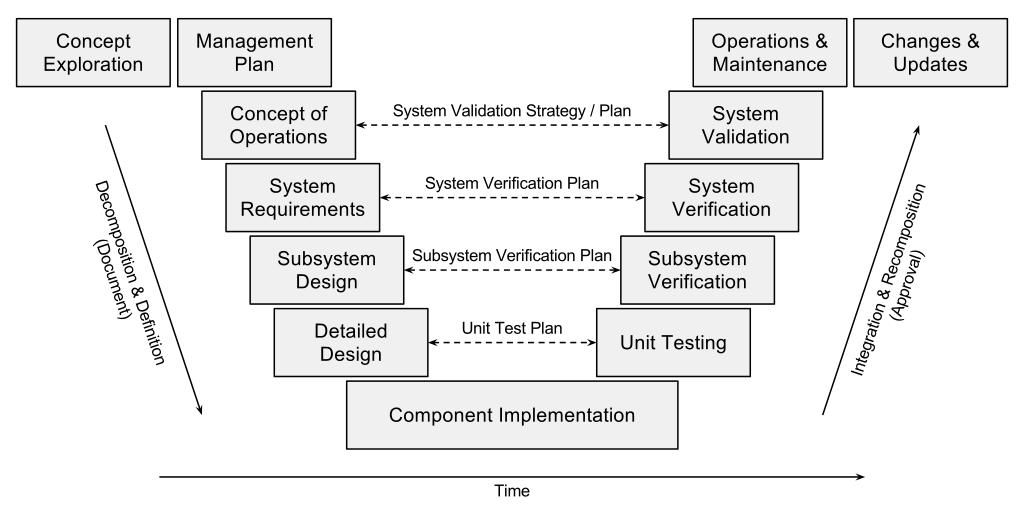
\includegraphics[width=\textwidth]{Thesis/Literature_Review/Lit Review Figures/sysengvee.png}
    \caption{Systems Engineering "Vee"}
    \label{fig:Systems Engineering "Vee"}
\end{figure}

Traditionally, the Systems Engineering process used a "document-based" approach, where documents are the primary artifacts available to stakeholders \citep{Delligatti}. These documents include requirement and traceability matrices, interface documents, concept of operation documents, and other unique documents in a wide variety of formats, such as Microsoft Excel sheets, Adobe PDF documents, Microsoft PowerPoint presentations, and digital drawings. As systems become more complex, the traditional document-based approach becomes challenging to maintain. Each document is manually generated, so file management and version control becomes problematic. It is difficult to know for sure if something is the current version or if it has been subsequently updated but located on some other file system or storage drive. Furthermore, any changes in one document, drawing, etc., must be also made in any other document that uses that same item. This system is prone to errors, inconsistencies, and difficulties maintaining an accurate representation of the entire system. MBSE provides a solution to these increasingly relevant problems. In MBSE, a system model represents the system and any information needed for documents can be found within this model. The model also makes it much easier to maintain consistency. If the modeler updates a component or interface in one area, it will be updated throughout the system wherever it appears. Traditionally, acquisition programs reviews will still require paper documents, but the necessary information for those can still be found within the system model during the transition from documents to system models. 

MBSE requires a modeling language, a modeling method, and a modeling tool \citep{Delligatti}. In this thesis, those are respectively the \abbreviationFull[Systems Modeling Language]{SysML}, the \abbreviationFull[Object-Oriented Systems Engineering Method]{OOSEM}, and the Cameo Systems Modeler tool.  

SysML is a standard modeling language, which added systems engineering functionality to the \abbreviationFull[Unified Modeling Language]{UML} that has been used extensively in Software Engineering for decades \citep{Delligatti}. SysML provides a language, or the definitions and notations for nine different diagram types to describe a complex system, many of which will be used in this Reference Architecture. SysML is expressed graphically through those diagrams, listed in Figure \ref{fig:SysML Taxonomy}, to show various system viewpoints. For example, a \abbreviationFull[Block Definition Diagram]{bdd} expresses system structure, and an Activity Diagram can show specific system activities. Within "blocks", further detail can be expressed on an \abbreviationFull[Internal Block Diagram]{ibd}. Further explanations will accompany their respective diagrams in Chapter \ref{analysisandresults}, but for now, it's important to know that SysML provides the language and is built into the modeling tool, described later in this chapter. 

The modeling method is the specific methodology used to ensure important design tasks have been accomplished and provides the general guidance, processes, or steps for the system design. This paper will focus on OOSEM, but there are other popular methods, such as the Weilkiens System Modeling (SYSMOD) method \citep{Weilkiens} and the IBM Telelogic Harmony-SE method \citep{IBM}.

\begin{figure}[H]
    \centering
    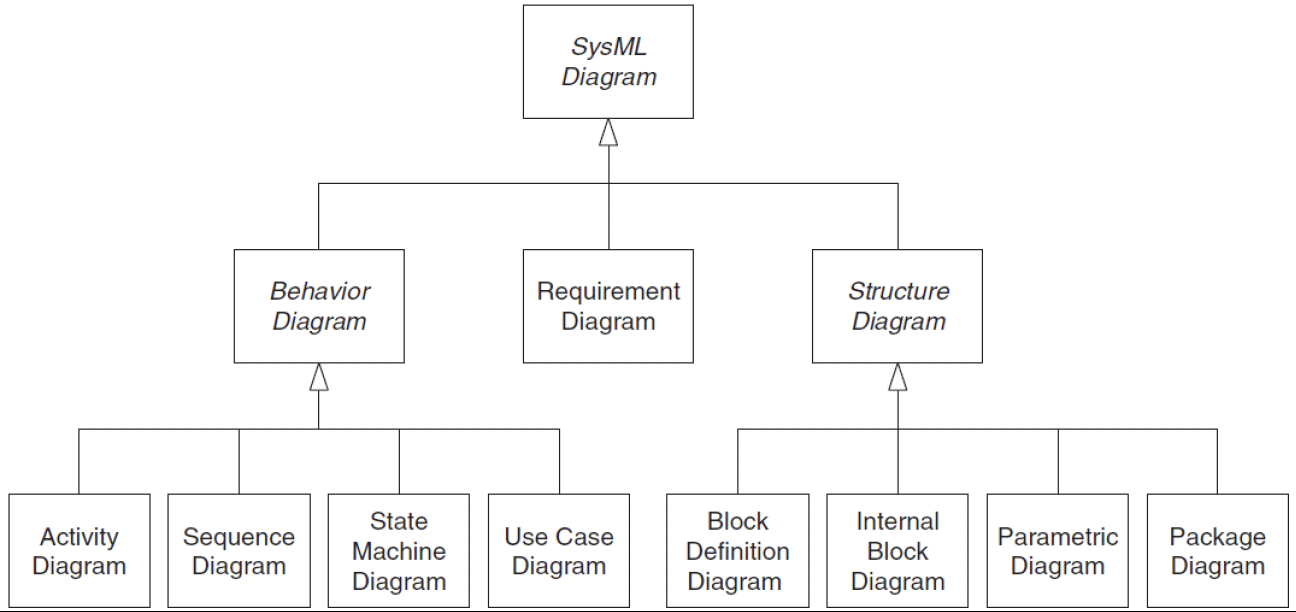
\includegraphics[width=5in]{Thesis/Literature_Review/Lit Review Figures/sysML taxonomy.png}
    \caption{SysML Taxonomy}
    \label{fig:SysML Taxonomy}
\end{figure}

OOSEM uses SysML in a top-down, model-based approach that leverages object-oriented concepts with traditional systems engineering methods to architect more flexible and extensible systems that can evolve with technology and changing requirements \citep{Estefan2008}. OOSEM was developed in part by Lockheed Martin Corporation as a method to capture and analyze requirements of complex systems, integrate with object-oriented software and hardware, and support system-level reuse and design evolution \citep{INCOSEhandbook}.

The primary OOSEM activities are similar to those in the traditional "Systems Engineering Vee" as described previously and are accomplished in an iterative fashion \citep{OMGwiki}. Similarly to the "Vee" method, the traditional technical management processes are still applied at each iteration.

The primary OOSEM steps are as follows \citep{Estefan2008}:
\begin{enumerate}
\item{\textbf{Analyze Stakeholder Needs:} Capture the "as-is" system and mission enterprise and identify gaps or issues. The "as-is" depiction helps develop the "to-be" system, and the gaps or issues can help drive mission requirements for the new system. OOSEM frequently uses measures of effectiveness for the primary mission objectives identified in this step.}
\item{\textbf{Define System Requirements:} Once the "as-is" system is defined and produces Mission Requirements, the system is modeled as a "black box" in a Mission Enterprise model. For example, instead of going deep into subsystem-level detail on a CubeSat, the entire CubeSat will be a "black box" that interacts with ground stations, other satellites, and the environment. This "black box" model allows for system-level activity diagrams and use cases to show how the "to-be" system will support the mission enterprise. This step helps derive system-level functional, performance, and interface requirements.}
\item{\textbf{Define Logical Architecture:} A "logical" architecture is created that captures key functions in logical blocks, allowing for specific components to be chosen later in place of the logical depiction.}
\item{\textbf{Synthesize Candidate Allocated Architectures:} From the logical architecture, create potential physical instantiations using value properties and selected components. Each component at this stage is then traced to system requirements in table or matrix form.}
\item{\textbf{Optimize and Evaluate Alternatives:} Trade studies or other analysis is conducted at this step among the candidate architectures. Parametric diagrams within the model or integrating other tools can simulate system performance with the chosen components so alternative solutions can be compared.}
\item{\textbf{Validate and Verify System:} Once a candidate architecture has been chosen from the alternatives, the system needs to be validated and verified to ensure the requirements are being met and that stakeholder needs are satisfied. This step uses inspection, demonstration, analysis, and test activities to validate and verify the system.}
\end{enumerate}

Finally, the modeling tool is how the language and method get put together. The modeling tool is a critical piece of software that builds an underlying model of the system that can be used to display many different viewpoints or diagrams, depending on what is needed. The system model in a modeling tool is comprised of model elements and relationships between those elements, and from those, diagrams can be generated. When the source element or relationship is modified or deleted, that change gets carried out throughout the entire model, in any and all diagrams those elements or relationships appeared. This effort utilized the Cameo Systems Modeler tool from No Magic Inc., but the process is tool-agnostic. Other tools are available on the market to accomplish the same goals with different user interfaces and feature sets. The Cameo Systems Modeler tool will be shown in model screenshots throughout this thesis. 


   	    \section{Reference Architectures}
        \label{RefArch}
   		Complex systems require a well-thought out architecture early on in the design process. The \abbreviationFull[Department of Defense]{DoD} attempted to manage the “Enterprise-level Architectures” and “Solution Architectures” throughout the department by publishing the \abbreviationFull[Department of Defense Architecture Framework]{DoDAF}. DoDAF defined an architecture as a “fundamental organization of a system embodied in its components, their relationships to each other and to its environment, and the principles governing its design and evolution over time \citep{DoDAF}.” This concept sounds reasonable, but system architects were not always available for every project that could benefit from a thought-out architecture. Reference Architectures help alleviate that problem by consolidating subject matter expertise and previous relevant architectures into digestible models that system designers can benefit from when creating a Solution Architecture \citep{Cloutier2010}. The DoD saw the benefits of Reference Architectures and put out a Reference Architecture Description in 2010, describing them as “an authoritative source of information about a  specific subject area that guides and constrains the instantiations of multiple  architectures and solutions \citep{RADescription}." 
\textcolor{red}{Reference the figure somewhere in this section too.}

\begin{figure}[!h]
    \centering
    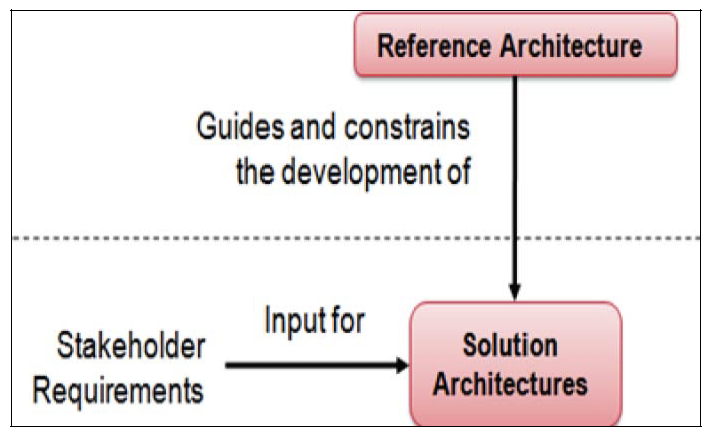
\includegraphics[width=3in]{Thesis/Literature_Review/Lit Review Figures/Ref Arc Purpose.png}
    \caption{Reference Architecture Purpose}
    \label{fig:Ref Arc Purpose}
\end{figure}

Cloutier suggests 2 key principles for Reference Architectures.

Principle 1: A Reference Architecture is an elaboration of company (enterprise) or consortium mission, vision, and strategy.   …facilitates a shared understanding about the current architecture and the vision on the future direction.

Principle 2: A Reference Architecture is based on concepts proven in practice. Preceding architectures can be mined for proven concepts.

Finally, Reference Architectures should have at least the following elements (cite...it was in Colombi's slide deck 23):
\begin{enumerate}
\item{\textbf{Strategic Purpose:} Goals, objectives, and a specific purpose or problem to be addressed}
\item{\textbf{Principles:} High-level foundational statements of rules, culture, and values that drive  technical positions and patterns}
\item{\textbf{Technical Positions:} Technical guidance and standards that must be followed by solution  architectures (maybe data vocabulary/ data model)}
\item{\textbf{Patterns (Templates):} Generalized representations (e.g., Viewpoints, Views, Diagrams, Products, Artifacts) showing relationships between elements specified in the Technical Position}
\item{\textbf{Vocabulary:} acronyms, terms, definitions}
\end{enumerate}

In summary, Reference Architectures can help systems engineers by providing a template, developed from years of experience, to aid in the systems engineering process. From the literature, it is clear that a Reference Architecture would be particularly useful for student groups designing a CubeSat.



   		\section{Existing Work}
        \label{Existing_Work}
   		There are many examples of Reference Architectures used in the commercial sector, but this section will focus on Reference Architectures that were clearly relevant to this effort. 

First, the \abbreviationFull[Small Unmanned Aircraft System]{SUAS} Reference Architecture developed at AFIT will be investigated. This is a relevant example as it fulfills the same general goals as the CubeSat Reference Architecture; namely, that it is for use in a design course series and is intended for students to use as a template for their design efforts. This SUAS Reference Architecture was started before this CubeSat effort and provides a useful baseline and inspiration, even if it is for a different domain. AFIT professors Dr. Jacques and Dr. Cox developed this architecture using Cameo Systems Modeler to describe a generic SUAS as described by the Army Research, Development, and Engineering Command, focused primarily on specific product output for the SUAS specialization track \citep{Jacques2019}. The SUAS Reference Architecture contains a Basic Ground Station Model, a Basic Multi-Rotor System Model, a Component Library, and sample build using the architecture.  The SUAS Reference Architecture is designed to allow students to easily build to a design specification from COTS components in the Component Library and test those designs using built-in parametric diagrams. These concepts will be applied to the CubeSat Reference Architecture as well, adapted for use in the spacecraft design course series. 
\begin{figure}[ht]
    \centering
    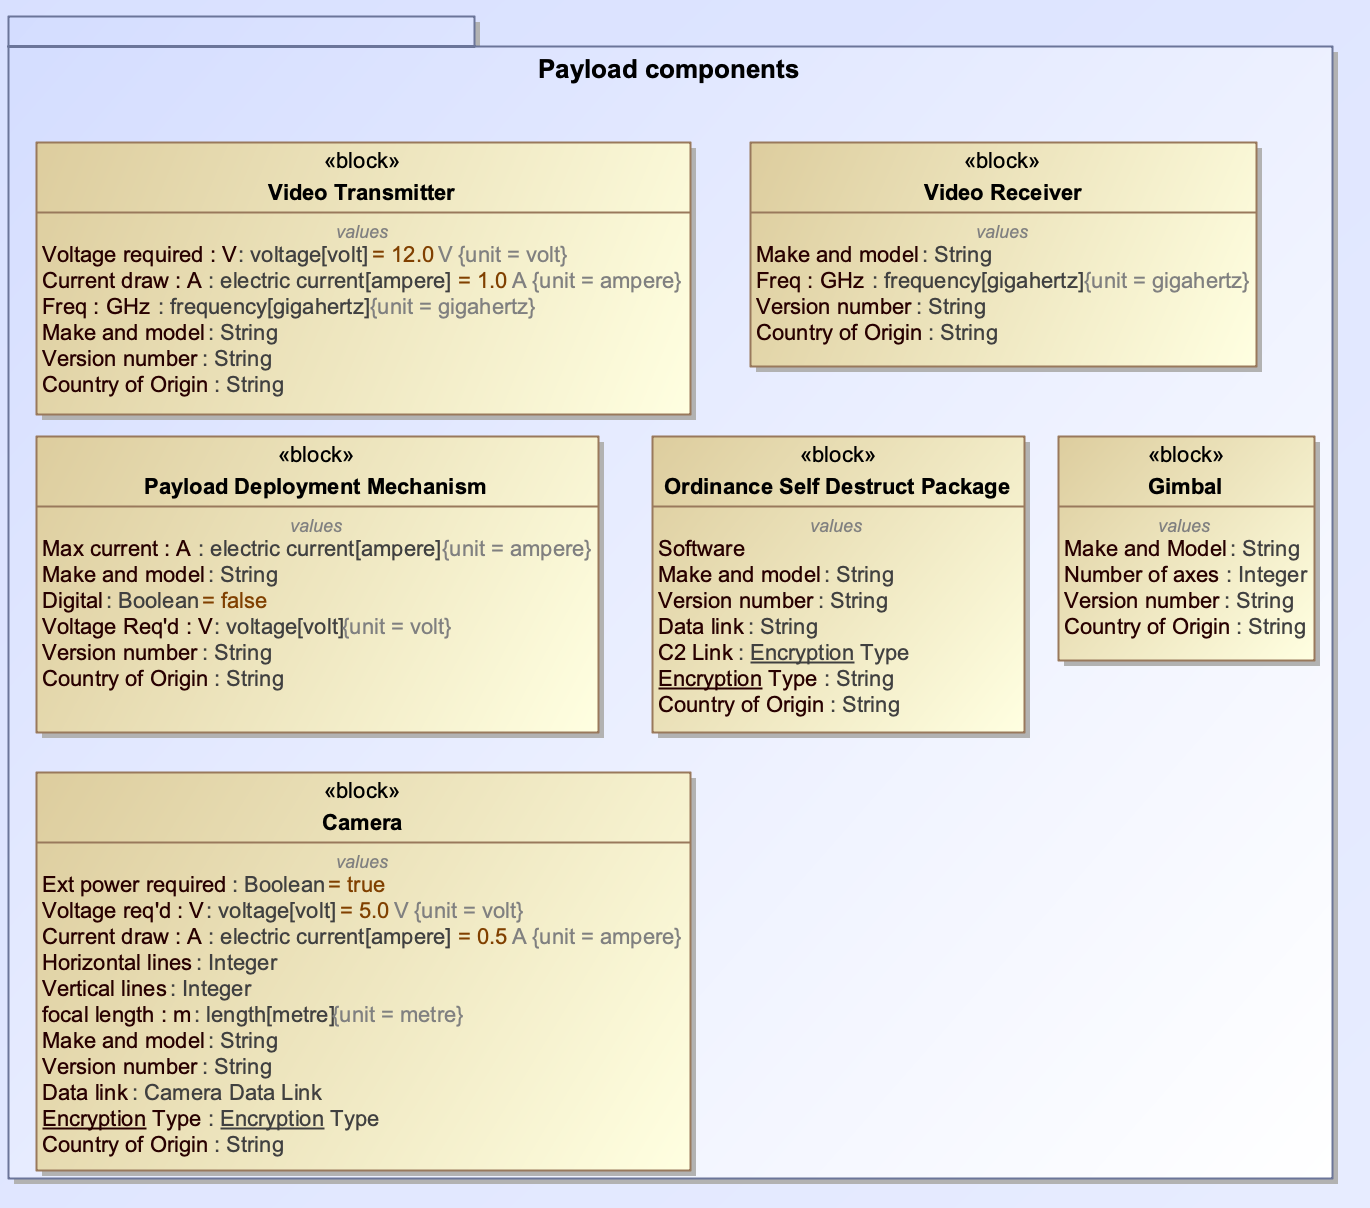
\includegraphics[width=\textwidth]{Thesis/Literature_Review/Lit Review Figures/suas component library.png}
    \caption{SUAS Component Library}
    \label{fig:SUAS Component Library}
\end{figure}



Jacques and Cox focused on the SUAS culture of rapid prototyping, and the Reference Architecture allows for designs to be developed at a much faster pace. The common template and vision provided through the model helps interdisciplinary teams design, build, and test SUAS systems with more time spent on producing a quality product, and less time spent designing the entire model from scratch \citep{Jacques2019}. Jacques and Cox captured their own extensive SUAS experience into their Reference Architecture, and the model will continue to be improved over time. Currently, it is being improved to streamline the cumbersome DoD Cybersecurity Risk Assessment process, using model elements to fill out required forms. The component library will also continually evolve as COTS components change. Figure \ref{fig:SUAS Component Library} shows a small section of their Component Library, providing blocks with value properties to start from. Figure \ref{fig:SUAS Organization} shows the SUAS Reference Architecture's top level organization, which this Reference Architecture will be modeled after for consistency. The component library, parametric diagrams, and general organization are useful in the development of the CubeSat Reference Architecture, but the spacecraft design course series has some unique differences that must be considered, such as instructor preferences and differing model scopes. 

\begin{figure}
    \centering
    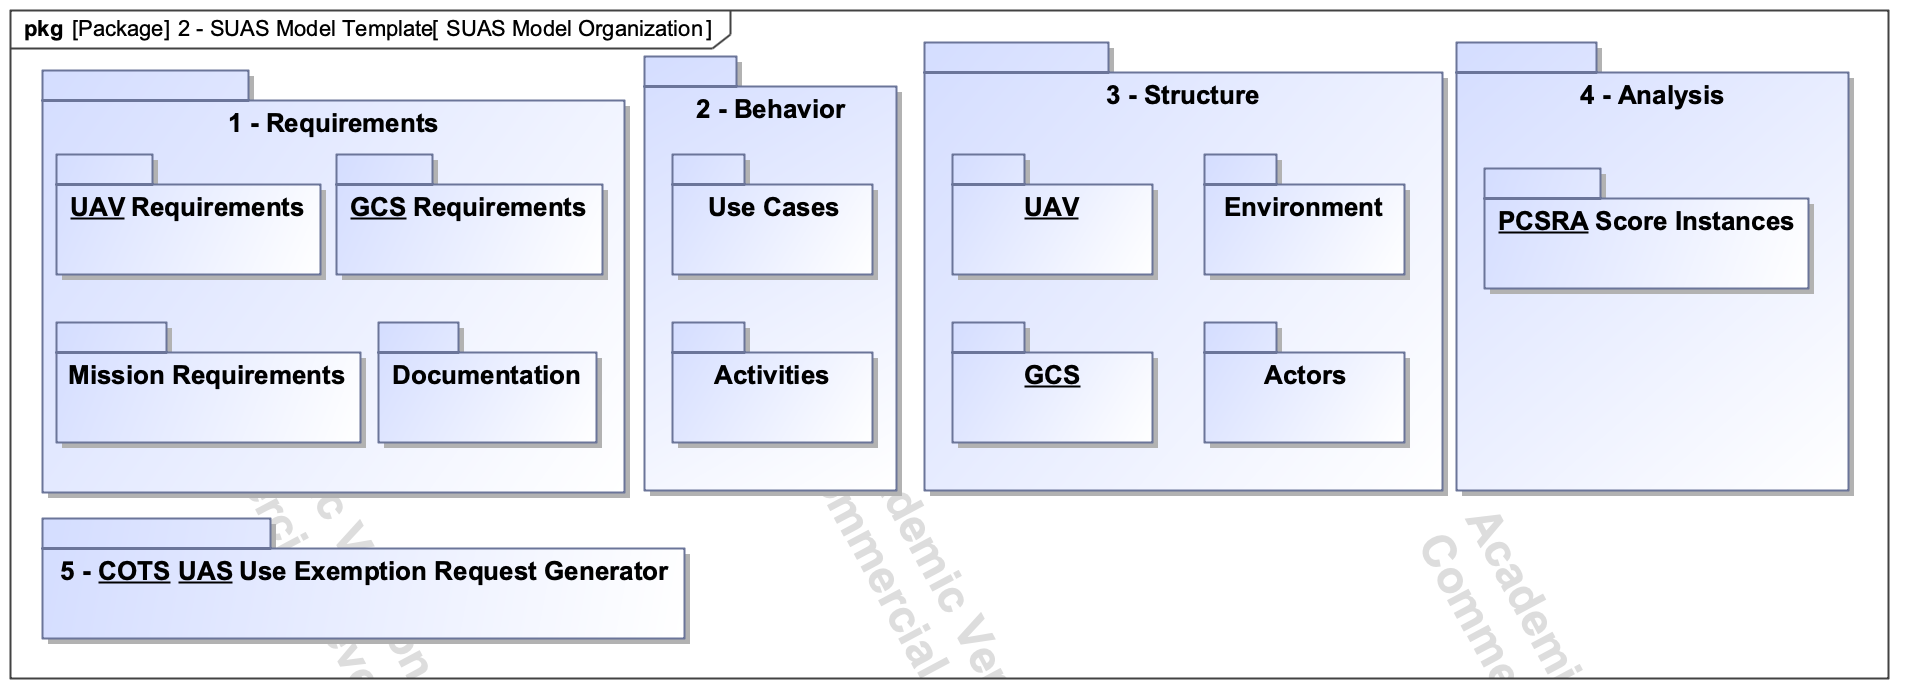
\includegraphics[width=\textwidth]{Thesis/Literature_Review/Lit Review Figures/suas organization.png}
    \caption{SUAS Organization}
    \label{fig:SUAS Organization}
\end{figure}

In the CubeSat domain, Kaslow and a group of Subject Matter Experts built a \abbreviationFull[CubeSat Reference Model]{CRM} as part of a partnership between the \abbreviationFull[Object Management Group]{OMG} and the \abbreviationFull[International Council on Systems Engineers]{INCOSE}. This CRM was intended to help CubeSat developers by providing logical, reusable architecture elements at a high level \citep{Kaslow2016}. Some sample diagrams are provided in their interim status updates \citep{CRM20,Kaslow2014,Kaslow2016,Kaslow2017,Kaslow2020,KaslowCRM3}, but the actual Cameo model was not available to investigate. This CRM describes three levels of architectural foundation that are necessary to capture the whole domain: the enterprise level, the space and ground segments, and the space and ground subsystems. Figure \ref{fig:CRM Domain} indicates the structure for the CubeSat domain as described by Kaslow et al.

\begin{figure}
    \centering
    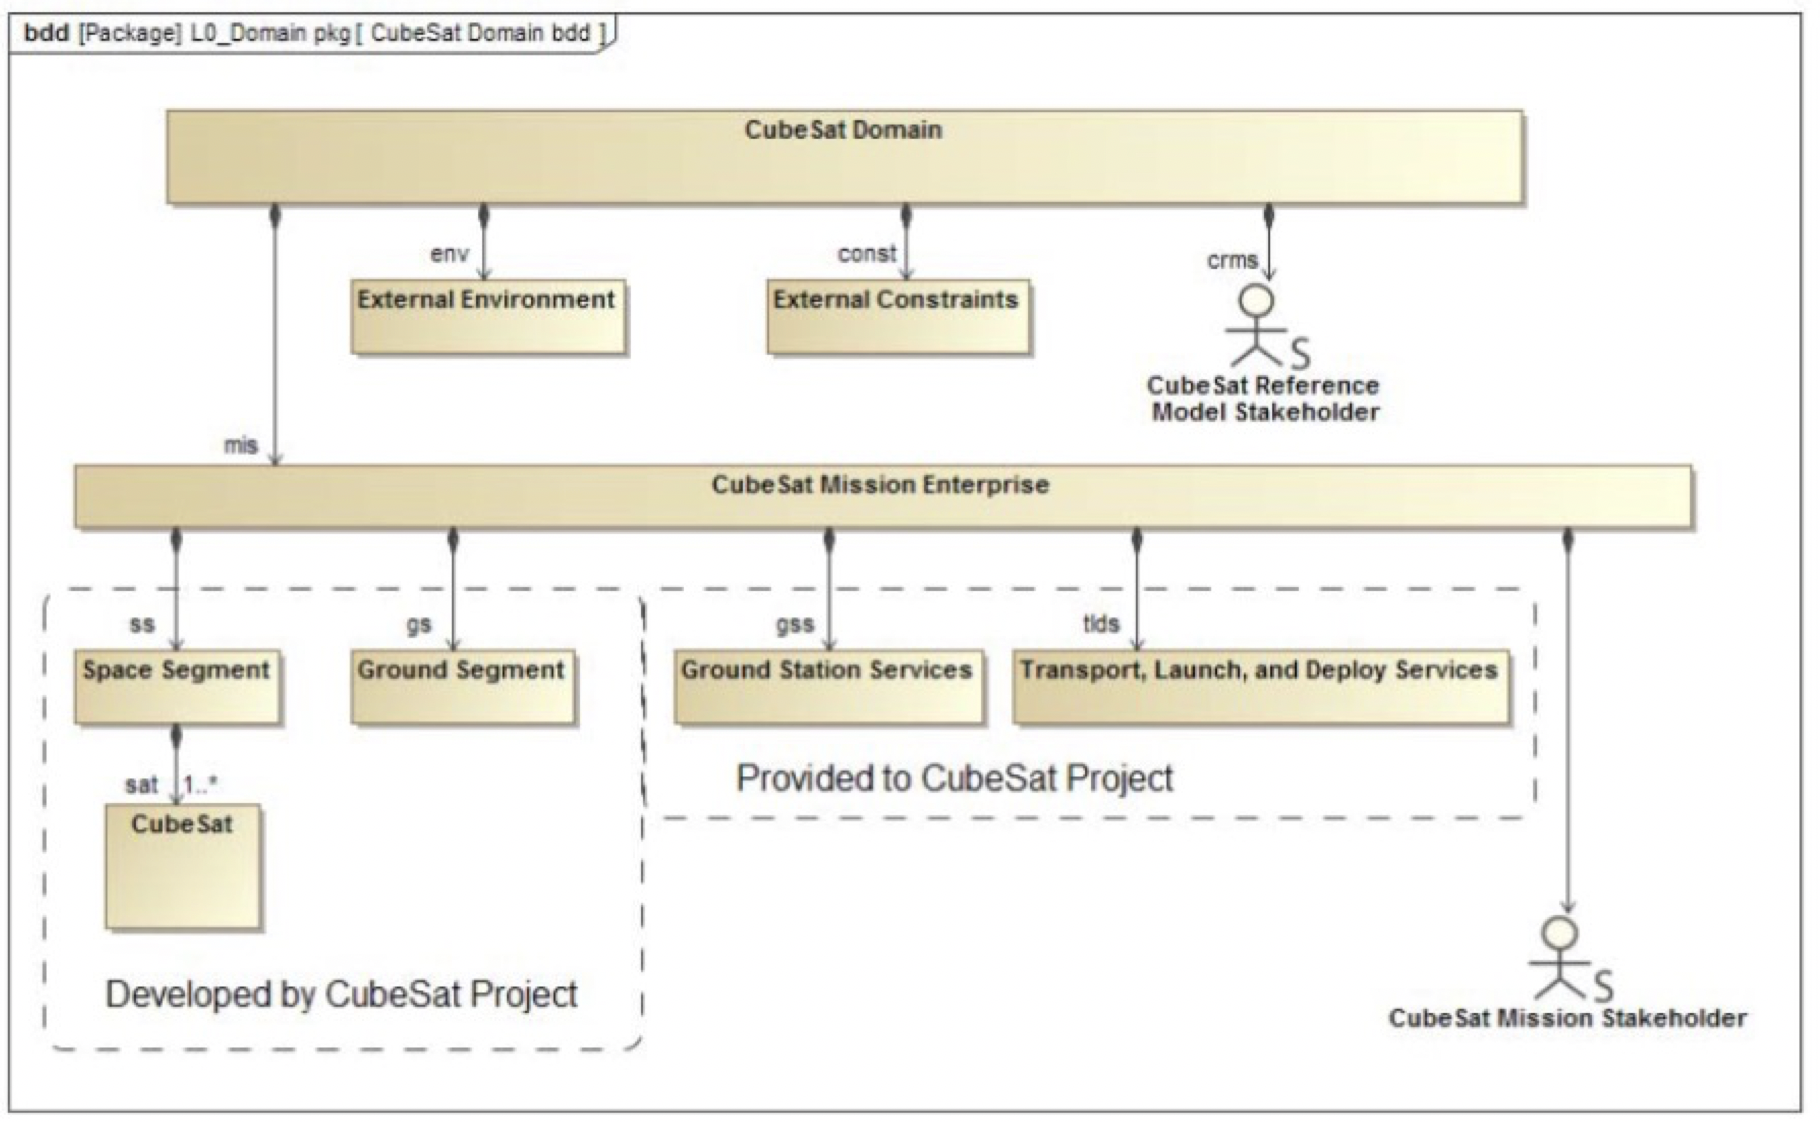
\includegraphics[width=\textwidth]{Thesis/Literature_Review/Lit Review Figures/CubeSat Domain.png}
    \caption{CRM CubeSat Domain}
    \label{fig:CRM Domain}
\end{figure}

Kaslow et al. used a block definition diagram to demonstrate the hierarchy of elements within the domain. They depict the CubeSat Mission Enterprise as being directly composed of a Space Segment, a Ground Segment, Ground Station Services, and Transport, Launch, and Deploy Services. Furthermore, they identified what must be developed by the CubeSat Project in greater detail, as shown by Figure \ref{fig:CRM RA Scope}.


\begin{figure}
    \centering
    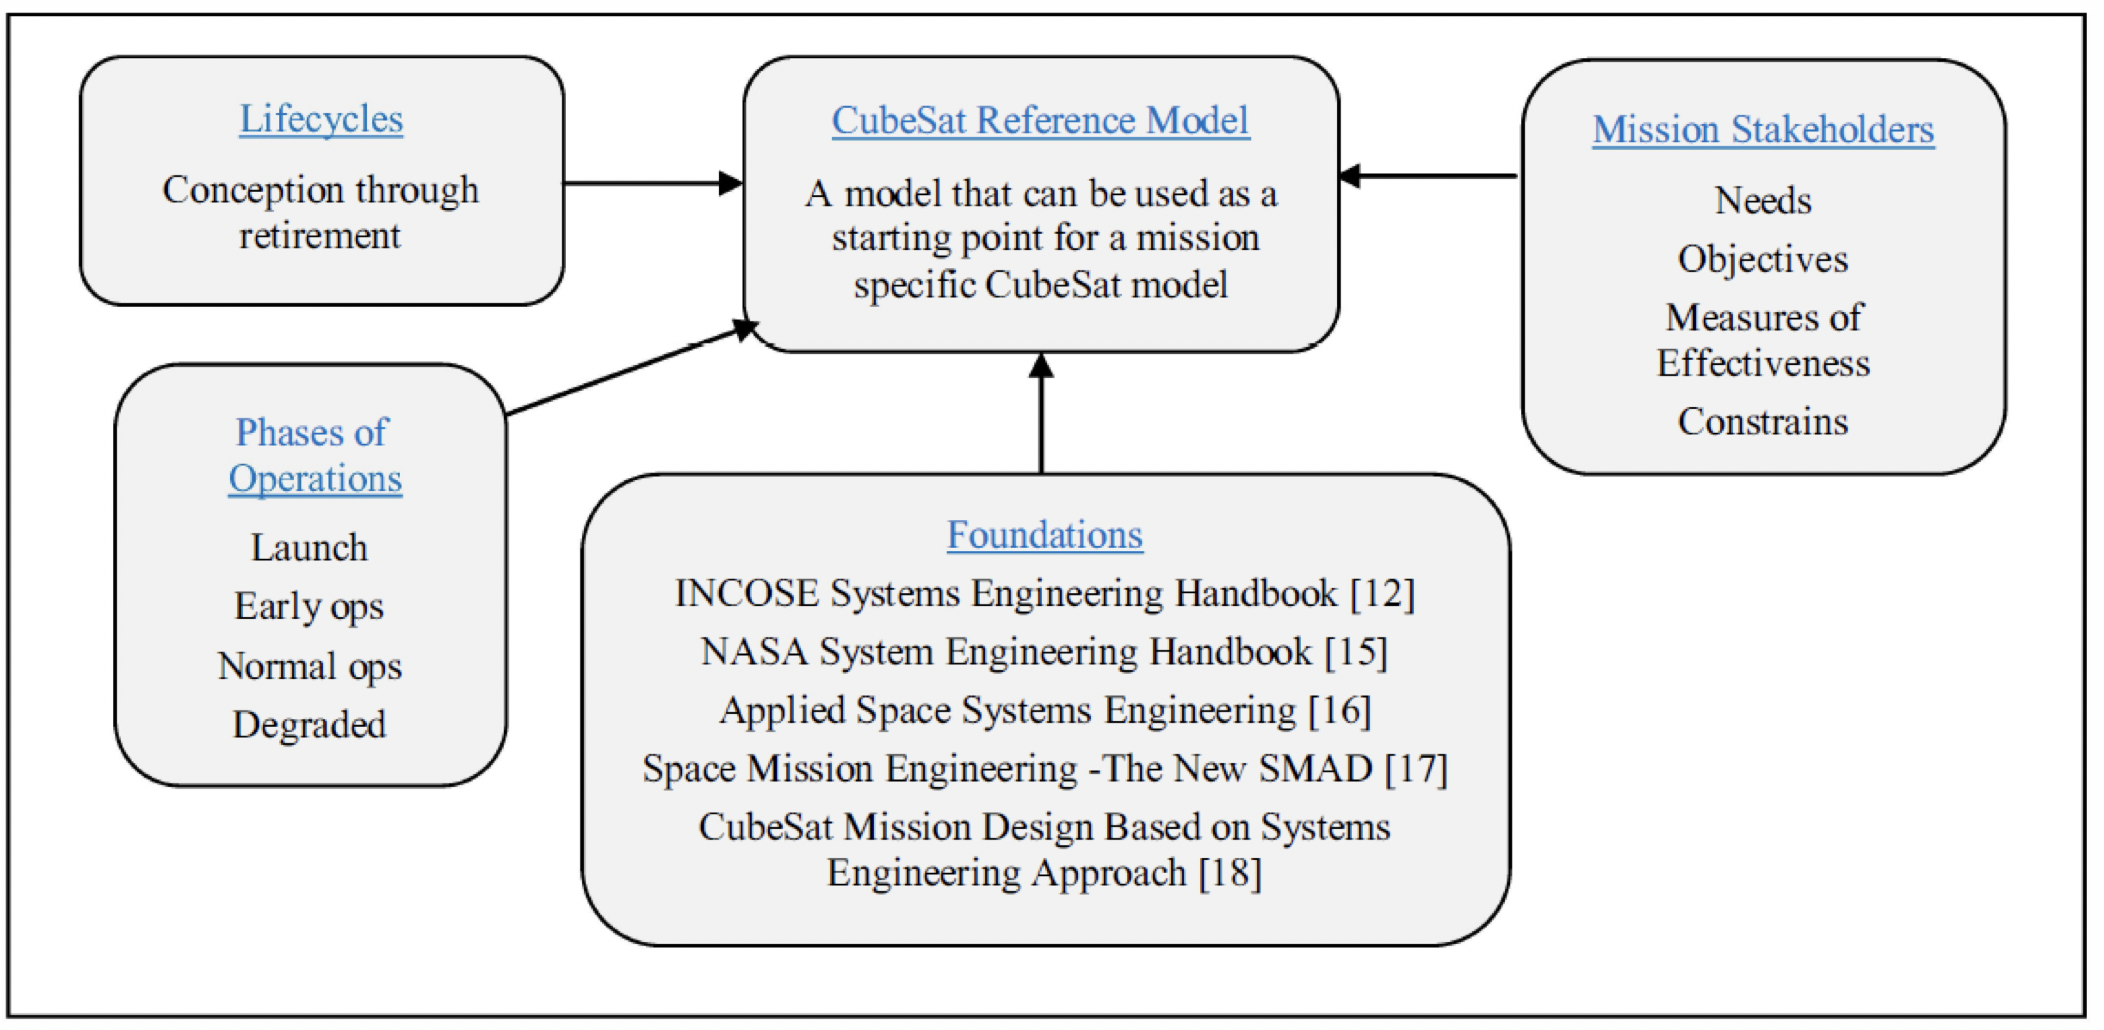
\includegraphics[width=\textwidth]{Thesis/Literature_Review/Lit Review Figures/CubeSat RA scope.png}
    \caption{CRM Scope}
    \label{fig:CRM RA Scope}
\end{figure}


\begin{figure}
    \centering
    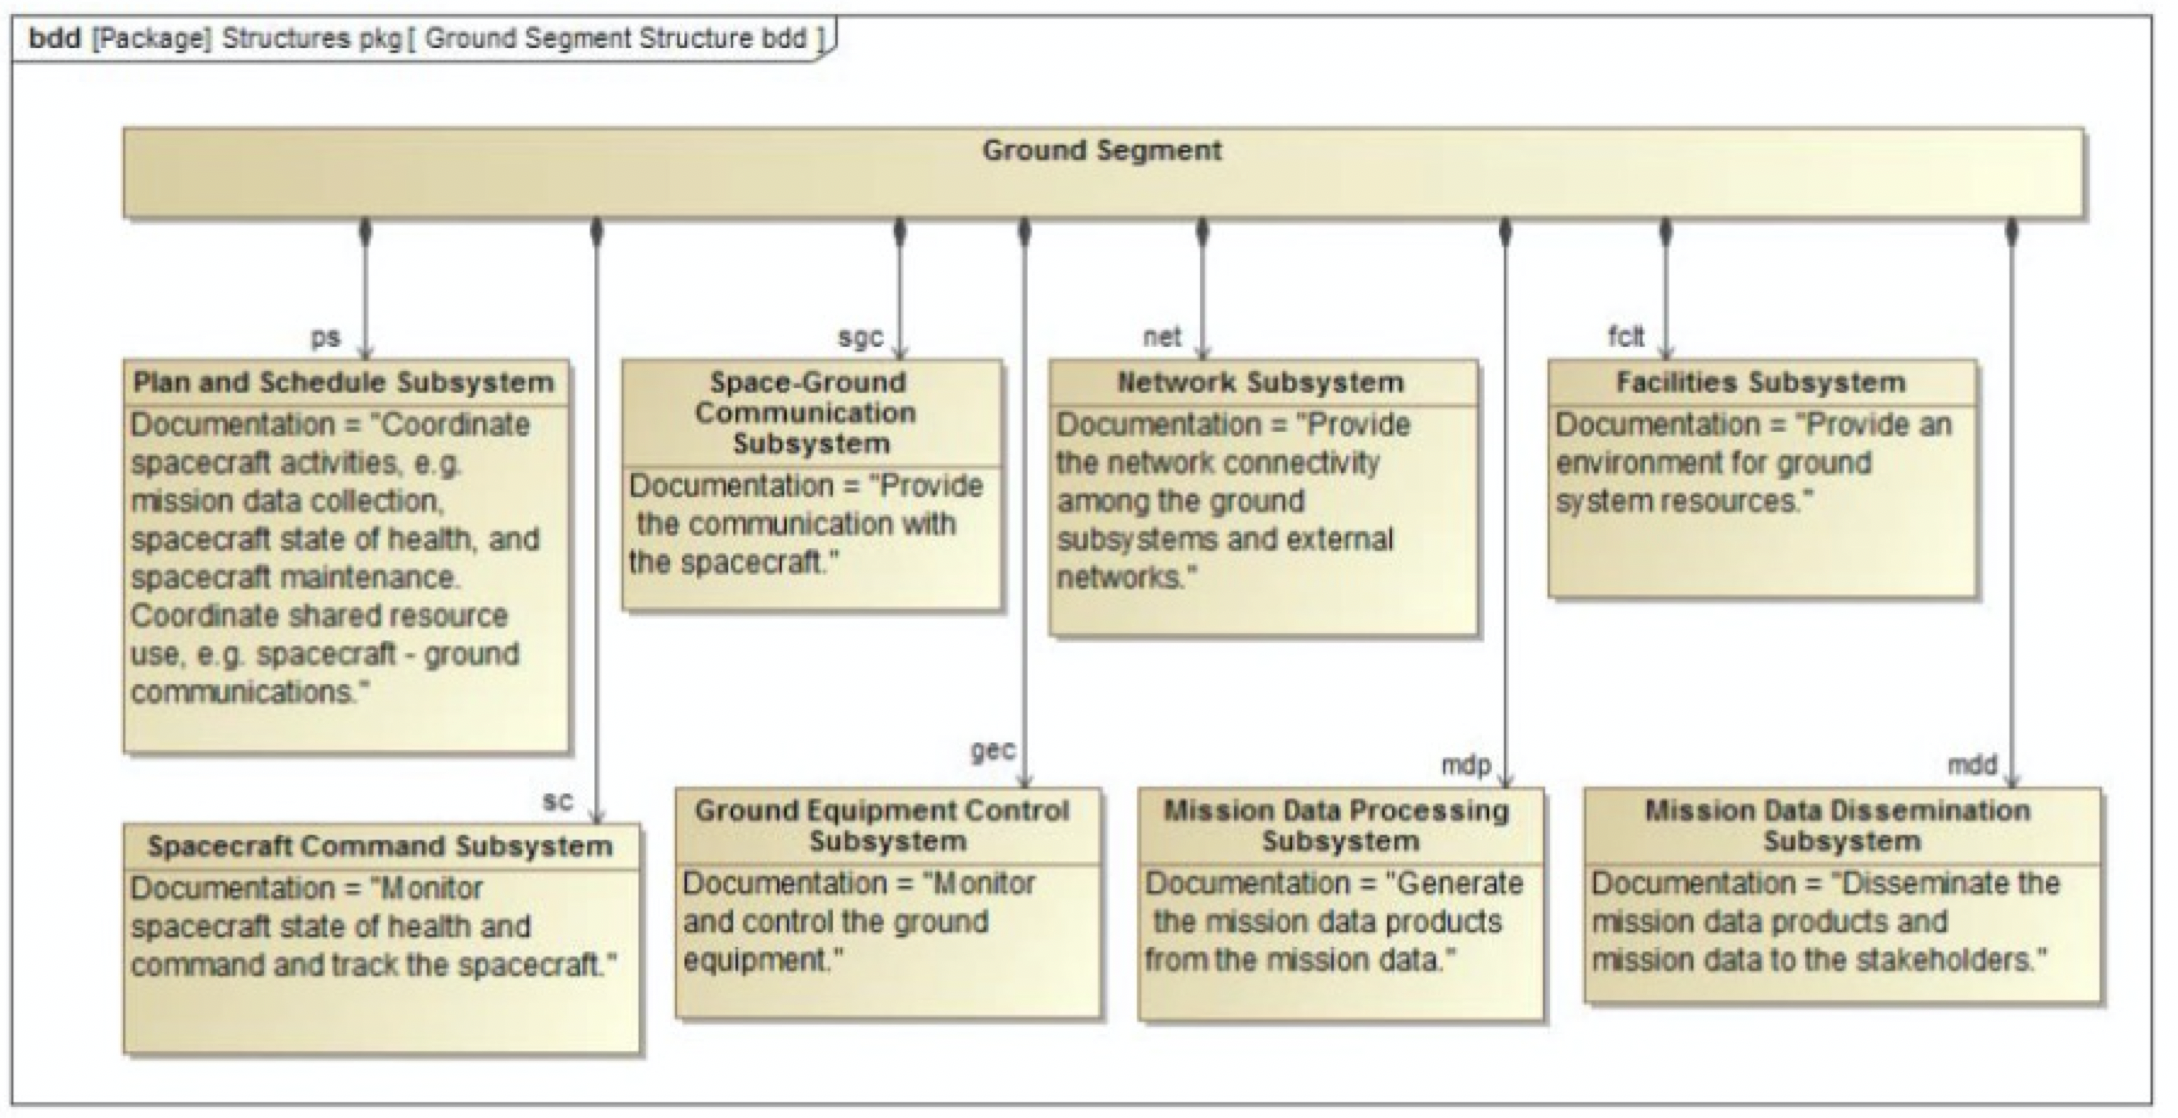
\includegraphics[width=\textwidth]{Thesis/Literature_Review/Lit Review Figures/CubeSat Ground Segment.png}
    \caption{CRM Ground Segment}
    \label{fig:CRM Ground Segment}
\end{figure}

\begin{figure}
    \centering
    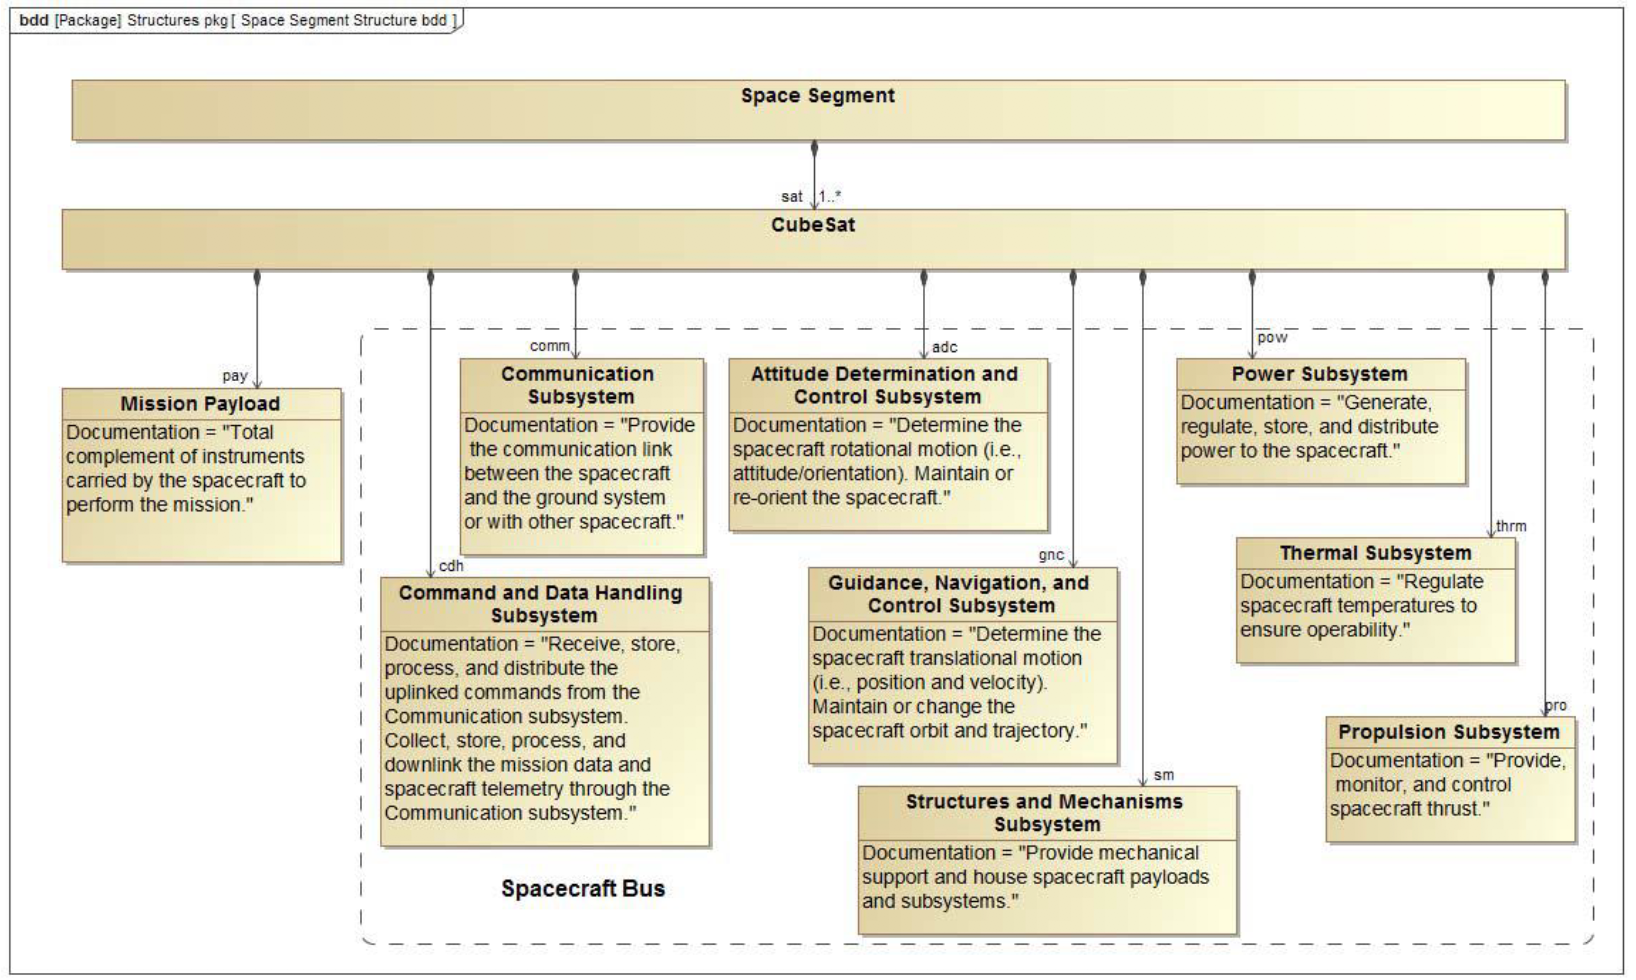
\includegraphics[width=\textwidth]{Thesis/Literature_Review/Lit Review Figures/CubeSat RA Space Segment.png}
    \caption{CRM Space Segment}
    \label{fig:CRM Space Segment}
\end{figure}


Kaslow et al. described all of the CubeSat subsystems and provided Block Definition Diagrams for the major views of a CubeSat, including each mission segment, as shown in Figure \ref{fig:CRM Ground Segment} for the Ground Segment and Figure \ref{fig:CRM Space Segment}.

Kaslow et al. determined that this logical architecture would provide guidance for CubeSat developers to begin to formulate their own mission specific architectures, knowing that their model did not have and could not have the specificity required to support every type of mission. It provided a top-level guide to how a CubeSat enterprise is organized, and some of the external stakeholders as well, as shown in Fig \ref{fig:CRM Stakeholders}. Their model is a starting point for mission specific teams to incorporate their unique knowledge to formulate their own reference architectures.

\begin{figure}
    \centering
    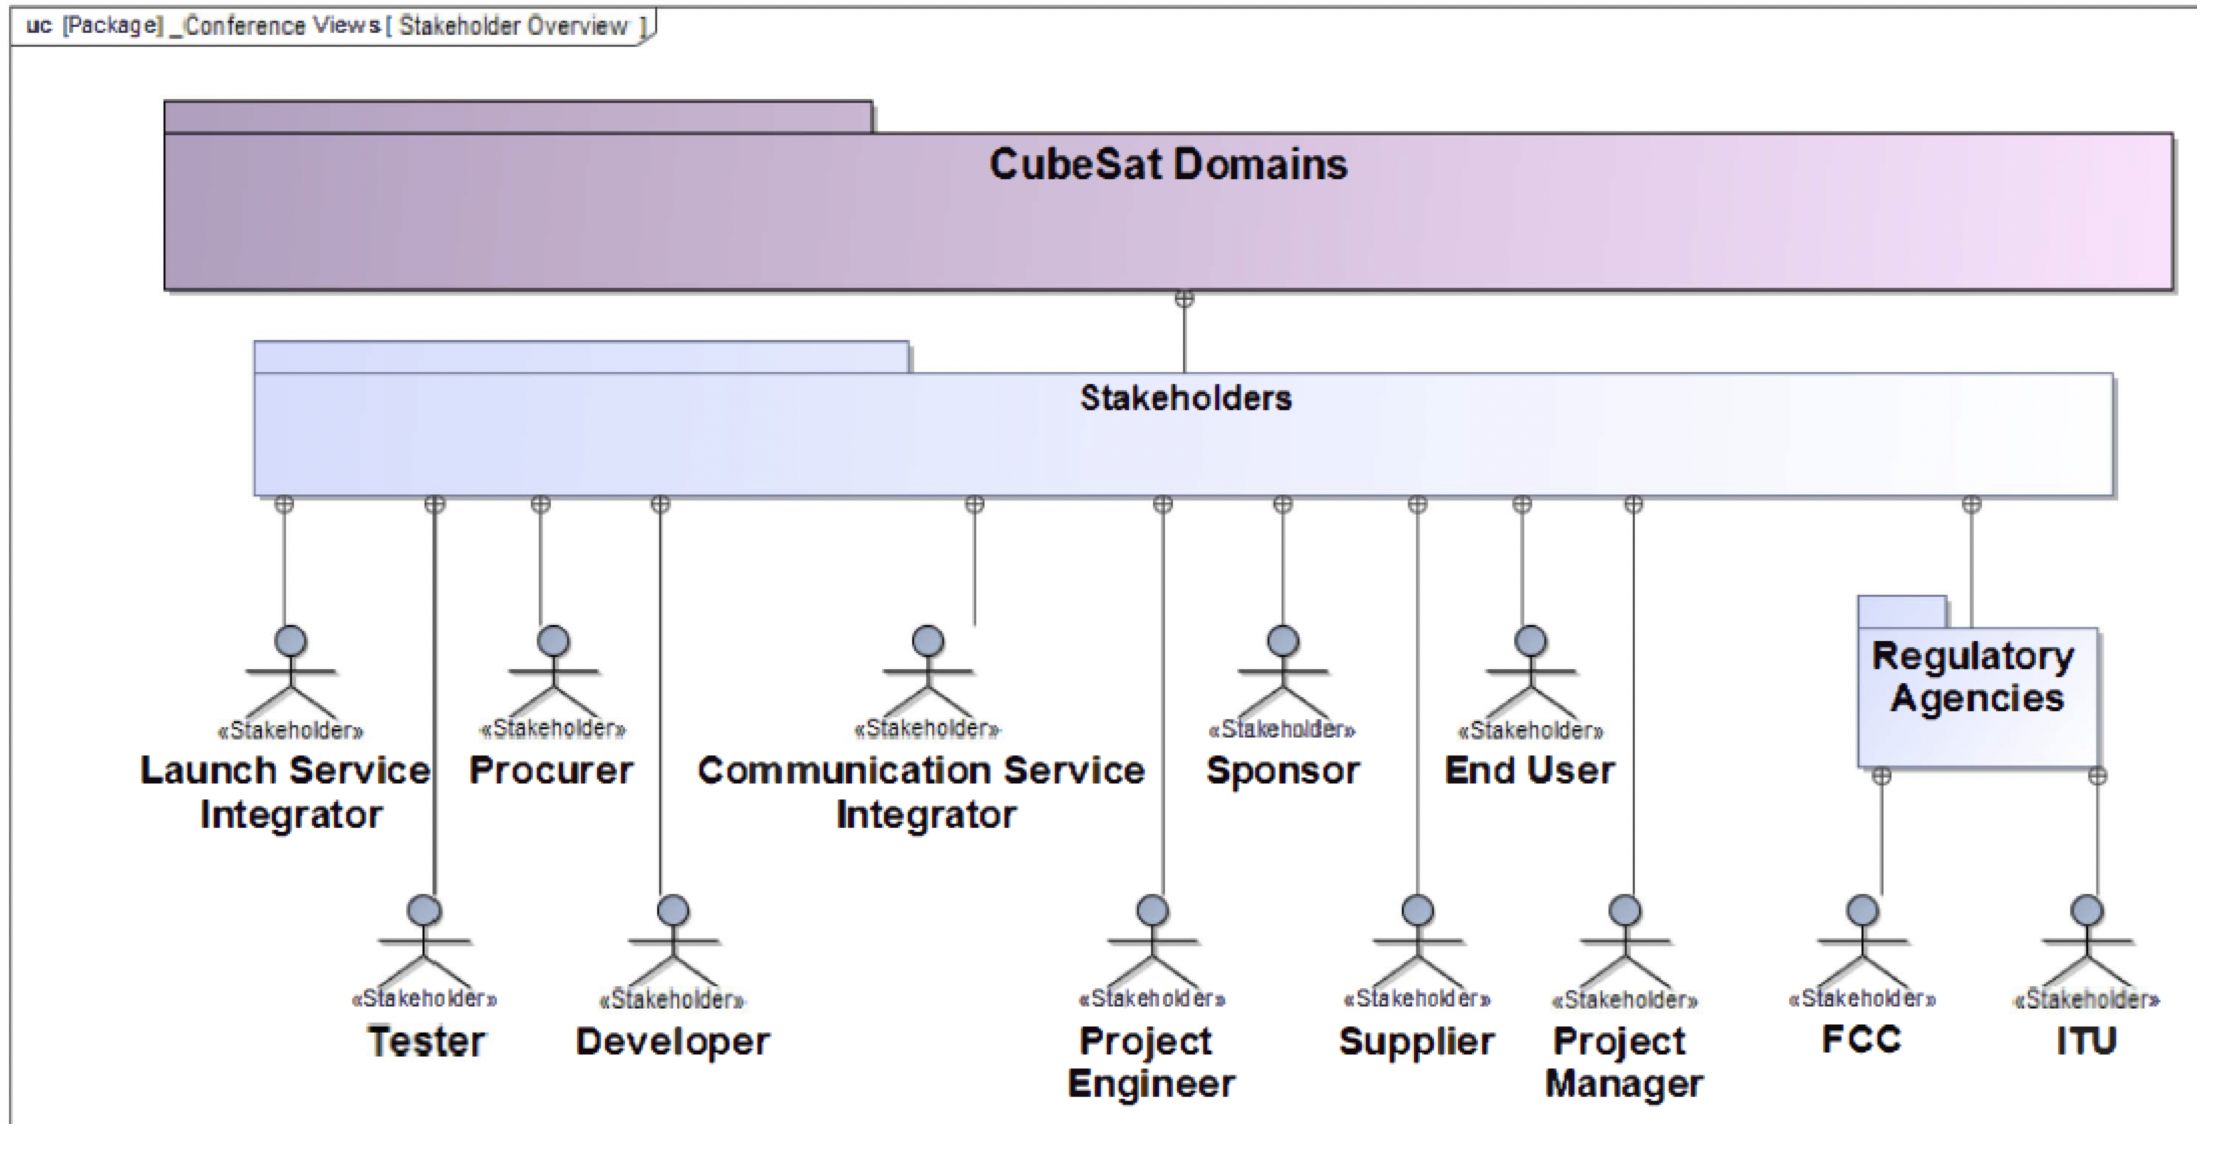
\includegraphics[width=\textwidth]{Thesis/Literature_Review/Lit Review Figures/CubeSat Stakeholders.png}
    \caption{CRM Stakeholders}
    \label{fig:CRM Stakeholders}
\end{figure}

After investigating the CRM status updates, however, the CubeSat Reference Model was missing much of the low-level details that was included in the SUAS Reference Architecture. A thorough reference architecture in this domain ought to include the high-level documentation and views of the CRM and the low-level component library and functionality of the SUAS reference architecture. 

Several other gaps exist that will be addressed in this thesis effort. First, the CRM is not designed for outputting traditional documents for system level reviews. There is no easy way to generate a \abbreviationFull[Concept of Operations]{CONOPS} document or \abbreviationFull[Operational Requirements Document]{ORD}, for example, and that is a desire for an AFIT CubeSat Reference Architecture. Second, the CRM does not appear to have a component library or a generic, intuitive system that can be easily adapted by students new to MBSE. Finally, the CRM does not appear to have sufficiently detailed value properties for the system to be useful for detailed mission analysis using MATLAB and STK. Students in the AFIT course series must design down to a very granular level of detail with many value properties for each subsystem in order to perform the required analysis and calculations. The CRM is quite useful though in examining what subject matter experts deem important for a CubeSat model and for their various subsystem internal block diagrams.

Another Reference Model that was investigated was the satellite model by Sanford Friedenthal \citep{FriedenthalArchitectingSpacecraft}. In his book, he walks through his version of a CubeSat model for the "FireSat II" mission, also using the OOSEM methodology and Cameo Systems Modeler. His book provides very helpful diagrams and best practices and will prove to be a key inspiration for this Reference Architecture. 

Should I even cite Luke Farrell's thesis? I didn't really use anything from his model...
   		
        \section{Summary}
        \label{Ch2Sum}
   		This chapter discussed the CubeSat context and explained the necessary MBSE and OOSEM concepts to understand the rest of this thesis. After the MBSE language, method, and tools were explained, Reference Architectures were defined, providing a template for the modeler to start from. Finally, current Reference Architectures were examined, including an AFIT-developed SUAS architecture and two existing CubeSat Reference Models. Gaps in these Reference Architectures were then identified that this thesis will attempt to solve. 
        
    \chapter{Methodology}
    \label{Methodology}

    	\section{Overview}
        \label{MethOverveiw}
        The purpose of this chapter is to highlight the current state of Reference Architectures, including some recent work in the CubeSat domain. To understand the context, this chapter will start by describing the CubeSat domain and the need for a CubeSat Reference Architecture. This chapter will also define key terms and explore gaps in the existing CubeSat models. Reference Architectures in the CubeSat domain are still a relatively new endeavor, but Reference Architectures in similar domains will be researched to learn lessons from those models as well. 

        
        \section{Summary}
        \label{Ch3Sum}
   		Chapter \ref{Methodology} described the status quo and inspirations for the Reference Architecture. Then, the process to create it was described, as well as the process for stakeholder input and model validation. 
        
    \chapter{Analysis and Results}
    \label{analysis}
    	\section{Overview}
        \label{subanalysis}
        The purpose of this chapter is to highlight the current state of Reference Architectures, including some recent work in the CubeSat domain. To understand the context, this chapter will start by describing the CubeSat domain and the need for a CubeSat Reference Architecture. This chapter will also define key terms and explore gaps in the existing CubeSat models. Reference Architectures in the CubeSat domain are still a relatively new endeavor, but Reference Architectures in similar domains will be researched to learn lessons from those models as well. 


    	\section{Section Name}
        \label{sectionname}
        % Section Name

MBSE tools and techniques were used to design the system from....

%\begin{figure}[!h]
%    \centering
%    \includegraphics[width=\textwidth]{Figures/funcdecomp.png}
%    \caption{caption text.}
%    \label{fig:functional_decomposition}
%\end{figure}

More text that references a Figure as such %Figure \ref{fig:behavior_decomposition} does not display a task layer. Additionally, the perceptor, hardware, deliberator, and coordinator provide functionality to the autonomous system which is displayed in Figure \ref{fig:perceptorhardwaredelib_functions}.

%\begin{figure}[!h]
%    \centering
%    \includegraphics[width=\textwidth]{Figures/behaviordecomp.PNG}
%    \caption{caption text}
%    \label{fig:behavior_decomposition}
%\end{figure}

More text

More figures

%\begin{figure}[!h]
%    \centering
%    \includegraphics[width=\textwidth]{Figures/LCMMessages.PNG}
%    \caption{The ....}
%    \label{fig:LCMconnections}
%\end{figure}

        
        \section{Summary}
        \label{Ch4Sum}
   		
This chapter presented the design and implementation of a....
        
    \chapter{Conclusion}
    \label{conclusion}
        \section{Overview}
        \label{conclusionoverview}
        The purpose of this chapter is to highlight the current state of Reference Architectures, including some recent work in the CubeSat domain. To understand the context, this chapter will start by describing the CubeSat domain and the need for a CubeSat Reference Architecture. This chapter will also define key terms and explore gaps in the existing CubeSat models. Reference Architectures in the CubeSat domain are still a relatively new endeavor, but Reference Architectures in similar domains will be researched to learn lessons from those models as well. 

    	
    	\section{Lessons Learned}
        \label{LessonsLearned}
        %Lessons Learned

Lessons learned section

























% \begin{table}[!t]
%     \centering
%     \caption{Summary of Lessons Learned and Future Recommendations.}
%     \begin{tabular}{ |p{5.5in}|} \hline
%     \textbf{SITL and Automated Testing} \\ \hline
%     - Determine if a physics model is used in Ardupilot SITL.  Incorporate more accurate models of the X-8 using JSBSim or similar tools.   Explore the effects of altering autopilot tuning parameters on swarm behavior. \\ 
%     - Automate the testing framework to reduce manual tasks for launching vehicles and algorithm code. \\ 
%     - Integrate automated analysis for testing to verify code changes, calculate flight statistics, or other relevant data. \\ 
%     - Introduce fault injection, degraded states, environment effects, and time delays in testing. \\ 
%     - Increase number of vehicles in the swarm. \\ 
%     - Add new variables to broadcast data in LCM messages such as autopilot mode and centroid calculation to better facilitate data analysis and grooming. \\ \hline
%     \textbf{Flight Testing} \\ \hline
%     - Verify required output data is present in log files during ground tests. \\
%     - Smaller way-point path to increase sorties per battery
%     - Higher $v_{max}$ for follower vehicles to allow gap closure to leader. \\
%     - Hold leader at way-point 1 before beginning tests to allow follower stability. \\
%     - Have all in `GUIDED' at conclusion of way-points to collect three-vehicle swarm stability data. \\
%     - Establish and follow start-up sequences. \\ \hline
%     \textbf{Hardware Changes} \\ \hline
%     - Update to Pixhawk 2 or PX4 autopilot. \\
%     - Incorporate RTK GPS for closer swarming capability. \\
%     - Change from BBB to ODROID for faster processing and to avoid clock resets during power-offs. \\ \hline
%     \textbf{LCM Tests} \\ \hline
%     - Synchronize log start times for more accurate message delay timing. \\ 
%     - Determine why some log times progressed at a higher rate. \\ \hline
%     \textbf{Algorithm Changes} \\ \hline
%     - Add or explore new rules for testing such as home location gravitation. \\
%     - Test for optimal parameter values, i.e. $b$, $r_{min}$, $u$. \\
%     - Alter code loop rates for different information streams. \\
%     - Incorporate predictive analysis of other swarm members to aid in degraded states. \\
%     - Introduce swarm damping parameter to reduce oscillations. \\
%     - Determine exact cause of unresponsive vehicles. \\ \hline
%     \textbf{Other} \\ \hline
%     - Broadcast UgCS telemetry via mesh network. \\
%     - Test mesh network concept for long ranges. \\
%     - Determine network bandwidth limitations for additional swarm members. \\ \hline
%     \end{tabular}
%     \label{tab:lessons}
% \end{table}
        
        \section{Future Work}
        \label{FutureWork}
        % Future Work

One of the primary goals for this CubeSat Reference Architecture was to establish the platform for future work. Some of that work has already begun, including an Integrated Mission Modeling Tool that uses the physical structure in the Reference Architecture to create detailed MATLAB Simulink and STK simulations for mission modeling. These tools will improve the fidelity of mission simulations and provide visual views of the orbits for ground contacts, while also simulating multiple payloads at once.

The Reference Architecture is meant to be improved and adapted over time. As new teams use the model, they will be creating new physical blocks for components they chose, and they will be creating new constraint blocks for analysis. These can be saved in the component library for future reuse, so over time, the component library can grow and contain more "plug and play" blocks. Eventually, the component library should have a variety of components for each subsystem to choose from, and there should be analysis blocks to tailor depending on the mission's requirements. 

There are also some gaps in the Reference Architecture that can be tackled by other researchers in the future. For example, this current iteration focuses on verifying subsystem level requirements with hardware tests, but most mission level or system requirements are not properly accounted for. This was due to the specific requirements of the Spacecraft Design Sequence at AFIT, but additional functionality can be built in to verify requirements at the mission or system level for teams who have a need for that information. Furthermore, only minimal risk functionality has been provided. Currently, a user can assign a risk level to a requirement, but there is no place to describe that risk or risk mitigation steps. 

        
        \section{Final Thoughts}
        \label{finalthoughts}
        % Final Thoughts here

This research used the Object Oriented Systems Engineering Method with SysML to create a CubeSat Reference Architecture. While originally intended to be used by students at AFIT in their Spacecraft Design Sequence, the model can be tailored to be used by other teams that have similar goals. 

This research delivered a variety of helpful tools for teams to use that makes their modeling efforts easier. Auto-populating tables and matrices, a library of parts and value properties to choose from, analysis patterns to tailor, and document generators will save time and hopefully improve the quality of CubeSat models going forward. Reports will also be more consistent and standardized according to stakeholder preference, and the work spaces provided encourage teams to use the model for storing all relevant data and analysis. Most importantly though, this Reference Architecture is cementing MBSE practices in teams who have limited experience with modeling tools, better preparing them for the future of spacecraft design.
        
    \appendix
     	
\backmatter
	\singlespace
    \bibliographystyle{plainnat}
    \bibliography{bibliography}
    \clearpage

    \date{March 2021}
\ReportDate{25--03--2021} 
\ReportType{Master's Thesis}
\DatesCovered{Sept 2019 --- Mar 2021}

\Title{A Reference Architecture for Rapid CubeSat Development}

\Author{Kelly, Sean R, Capt}

\PerformingOrg{Air Force Institute of Technology\\[-1pt]
    Graduate School of Engineering and Management (AFIT/EN)\\[-1pt]
    2950 Hobson Way\\[-1pt]
    WPAFB OH 45433-7765}

\POReportNumber{AFIT-ENV-MS-21-M-240}

\SponsoringAgency{Air Force Institute of Technology\\[-1pt]
WPAFB OH 45433\\[-1pt]
DSN 785-6565, COMM 937-255-6565\\[-1pt]
}

\Acronyms{AFIT/ENV}
%\SMReportNumber{}
\DistributionStatement{DISTRIBUTION STATEMENT A:\\
\MakeUppercase{Approved for Public Release; distribution unlimited.}}

\Abstract{The CubeSat class of nanosatellites has lowered the barrier of entry to space and has rapidly gained popularity in recent years. To successfully design a CubeSat system in a rapid cycle conducive to academic timelines, a Reference Architecture geared towards University CubeSat development would be helpful. A Reference Architecture would speed up the development process by providing a template, capturing previous work and lessons learned from subject matter experts, providing a framework to focus on the CubeSat’s design rather than the fine details of modeling software. A Reference Architecture can also add functionality that student teams could use and improve over time, such as pre-built analysis functions and a library of components to choose from. This thesis presents a CubeSat Reference Architecture designed to meet these needs and explores its unique features, diagrams, and custom libraries. The CubeSat Reference Architecture was validated by relevant course instructors and is being used by a cohort of students in the Spacecraft Design Sequence at AFIT.}

\SubjectTerms{Reference Architecture, CubeSat, MBSE}

\NumberPages{108}
%\ReportClassification{}
%\PageClassification{}
%\AbstractClassification{}
\AbstractLimitation{U}

\ResponsiblePerson{Dr. David R. Jacques, AFIT/ENV}

\RPTelephone{(937) 255-3636, x3329; david.jacques@afit.edu}

\MakeRptDocPage

\end{document}
